\chapter{Marco teórico}
En esta sección entramos en detalle el marco conceptual y el marco tecnológico. En la primera sección se verán los modelos de enseñanza y la teoría sobre la enseñanza de programación, así la forma de aprovechar los videojuegos para la enseñanza, sus ventajas y la forma de enseñanza que estos proveen, y la metodología de software a usar y sus artefactos. En la segunda sección discutimos de tecnologías aptas para la realización del proyecto.

\section{Marco Conceptual}

\subsection{Modelos de enseñanza}
Pueden ser definidos como \enquote{el conjunto de lógico y unitario de los procedimientos didácticos que tienen a dirigir el aprendizaje, incluyendo la presentación y la elaboración de la materia hasta la verificación y competente rectificación del aprendizaje} \cite{metodos_ensenanza}. Para Jean Pere hay tres modelos principales:

\subsubsection{Modelo tradicional}
En este modelo la enseñanza el papel del profesor es explicar claramente y que expongan el tema de manera progresivamente hasta el nivel de profundidad deseado. Si aparecen errores en los resultados del alumno, es porque este ultimo no  tuvo la actitud de aprender. El alumno es un individuo pasivo en este modelo.

\subsubsection{Modelo conductista}
En este modelo el profesor incentiva el alumno al aprendizaje (ej. calificaciones, el aprendizaje se recompensa con buenas calificaciones), sin embargo, aunque se evalúa el desempeño del alumno, nada asegura que el comportamiento externo corresponda con el mental como sería el aprendizaje superficial o la memorización.

\subsubsection{Modelo constructivista}
La enseñanza en este modelo es vista como una actividad critica, en este el profesor es visto como un profesional autónomo que investiga reflexionando sobre la practica de esta, el error es visto como una parte vital del aprendizaje, o \enquote{aprender es arriesgarse a errar} \cite{metodos_ensenanza}.

\subsection{Métodos de aprendizaje}
Se refiere a la diferente de la forma en la que las personas aprenden de mejor manera. Existen 4 métodos \cite{metodos_aprendizaje}: 
\begin{itemize}
    \item Aprendizaje auditivo, las personas que aprenden mejor de este método se les hace mas fácil escuchar y les funciona actividades como acudir a conferencias, charlas o ver documentales relacionados.
    \item Aprendizaje visual, estas personas aprenden mejor con diagramas o esquemas.
    \item Aprendizaje táctil, estos aprenden mejor con la práctica.
    \item Aprendizaje cinestético, aquellos que aprenden moviéndose o gesticulando, para estas personas les es útil es su aprendizaje ir a museos o realizar representaciones de obra de teatro.
\end{itemize}

\subsection{Enseñanza de programación}
Enseñar programación es una actividad compleja, porque incluye una variedad de dominios que son difíciles y que se sobre-empalman en la practica \cite{Robins2003}. Boulay define cinco de estos dominios:
\begin{itemize}
    \item Orientación general, que es lo que se puede realizar con un programa.
    \item La maquina notacional, un modelo de mental del funcionamiento de la computadora, dado por las estructuras del lenguaje de programación usado.
    \item Sintaxis y semántica del lenguaje de programación usado.
    \item Estructuras y planes, como se traslada el problema a las capacidades del lenguaje de programación
    \item Pragmáticos, las actividades planificación, desarrollo, pruebas, \textit{debugging}, etc. 
\end{itemize}
Todo esto que crea un \textit{shock} inicial en los estudiantes al tener que enfrentarse con diferentes tipos de dificultad al mismo tiempo, en muchos métodos de enseñanza de programación se intenta dar vuelta alrededor de esto mediante ejercicios diseñados para reducir la complejidad de la actividad al reducir su alcance en cuanto a las habilidades requeridas o en su defecto, generando suficiente \textit{engagement} para contrarrestar la tediosidad con trabajo interesante como manipulación de vídeo, imágenes o audio.

\subsubsection{Instrumentos didácticos}
Algunos de los instrumentos didácticos que se han probado y han mostrado efectividad para enseñar programación son los siguientes \cite{Wilson2019} \cite{Brown2018}:
\begin{enumerate}
    \item Una investigación \cite{Brown2018} menciona que los estudiantes no recuerdan las demostraciones, incluso recuerdan erróneamente el funcionamiento del programa. Se recomienda hacer que los estudiantes hagan alguna predicción y que el resultado de esta sea publica, se especula que el hecho de estar el alumno expuesto públicamente a que se equívoco hace que el ponga mas atención y reflejar sobre su entendimiento.
    \item Se encontró que estudiantes que manipulan imágenes, audio y vídeo temprano en el curso de programación aumentan retención y sus las posibilidades de que continúen su curso. Aunque mencionan que las investigaciones resaltan que no importa el contexto, un ejercicio de ordenar números no es menos recordado que uno de ordenar calificaciones. Lo importante es pasar a trabajo interesante para el alumno lo mas pronto posible.
    \item Realizar evaluaciones cada 10 - 15 minutos. Permite alentar la velocidad de la clase a la velocidad en la que los estudiantes aprenden. Se pueden hacer actividades como:
        \begin{enumerate}
            \item Contestar una pregunta de respuestas múltiples
            \item Escribir algunas lineas de código
            \item Predecir que hace el código en pantalla
            \item Seguir el orden de ejecución del programa
        \end{enumerate}
    \item Así como evitar solo programar, para niveles principiantes la actividad de programar incluye recordar sintaxis, ejercicios que reduzcan la carga cognitiva a un concepto en especifico son ideales, una forma alternativa es ofrecer las lineas de código de la solución fuera de orden para practicar flujo de control.
    \item Usar una variedad de ejercicios:
        \begin{enumerate}
            \item Preguntas de respuesta múltiple
            \item Arreglar, terminar o extender programas existentes
            \item Seguir el orden de ejecución del programa
        \end{enumerate}
    \item Peer programming, tener dos programadores trabajando juntos en una sola computadora, donde una persona escribe el código mientras la otra dirige a la primera en el diseño y configuración del código. Tiene las ventajas de mejorar retención, rendimiento y aumenta confianza del alumno en si mismo \cite{ncwit}.
\end{enumerate}

\subsubsection{Estrategias de los métodos para enseñar programación}
Existen varias estrategias para enseñar programación, por lo regular son usadas varias a la vez por los docentes \cite{Szlavi2003}.
\begin{enumerate}
    \item Orientado a algoritmos. Consisten en enseñar al alumno tipos de problemas generales y su solución algorítmica, de forma que el alumno pueda encontrar la forma de pasar un problema a teoremas de programación.
    \item Orientado a \textit{data}. El enfoque principal es convertir los problemas a tipos de datos y enseña a los alumnos los algoritmos para trabajar los tipos de datos resultante.
    \item Orientado a la especificación. A este le importa el desarrollo de especificación formal, del cual se crea el algoritmo y el código siguen al pie de la letra este.
    \item Orientado a problemas. Asevera que el proceso de programar no se puede dividir en distintas actividades. Inicia con problemas a resolver y las herramientas son dadas al estudiante según sea su demanda.
    \item Orientado al lenguaje. Enseña un lenguaje en particular, su inconveniente es cuando el estudiante cambia de lenguaje de programación hay información dependiente del lenguaje que es complicada de transportar a nuevos lenguajes.
    \item Orientado a las instrucciones. Mas abstracto al anterior, trata de enseñar las bases de un tipo de lenguajes de programación.
    \item Orientado a matemáticas. Los problemas a resolver se toman de las matemáticas, un problema que tiene es que al enfocarse en temas específicos de las matemáticas se hace al lado la enseñanza de programación y quedan huecos de conocimiento.
    \item Orientado al hardware. Nace de la idea de que no se puede entender un lenguaje de programación sin tener conocimientos de lenguaje ensamblador o lenguaje maquina, el diseño de algoritmos y tipos de datos normalmente queda de lado. Considerada obsoleta.
    \item Basado en modelos. El estudiante aprende mediante el estudio de programas ya creados. Este experimenta el programa evaluando los resultados obtenidos e iterando hasta llegar a la solución esperada. Se considera un método obsoleto y no útil para enseñar a escala.
\end{enumerate}

\subsubsection{Métodos de enseñanza de programación}
Hay varios métodos de enseñar programación, pensados para tratar de reducir la complejidad de la programación con ayuda de compañeros, trabajo interesante y material didáctico fácilmente consultable. Estos son algunos métodos usados \cite{mohorovic}:
\begin{itemize}
    \item Basado en problemas, este método obtiene \textit{engagement} de los estudiantes al resolver problemas que los profesionales del área se encuentran todos los días
    \item Basado en \textit{puzzles}, enseñan en el estudiantes habilidades de pensamiento critico y solución de problemas. Los problemas deben poner un desafió al estudiante sin alguna solución obvia, pero con la promesa de que se puede resolver.
    \item Programación por pares, tratado anteriormente, un estudiante es el conductor que escribe el código, y el navegador que revisa su trabajo y guía el diseño.
    \item Lecturas pre-grabadas, pensadas para suplementar las lecturas, ofrecen grabaciones de las diapositivas con notas de forma que los estudiantes puedan revisarlas a su propio ritmo cuando queden dudas.
    \item Programación orientada a juegos, ayuda a los estudiantes a aprender conceptos abstractos de programación explorando y programando pequeños juegos, se mueve lo que normalmente seria programas de consola a lógica de juego que enseñen los mismos conceptos.
\end{itemize}

\subsubsection{Métodos subyacentes}
PRIMM es un método de enseñanza de programación que incorpora discusión e investigación de muestras de código, esta diseñado para resolver el problema de que los estudiantes tengan que escribir programas antes de que tengan la habilidad de leerlos, consiste de 5 elementos \cite{Sentance}:
\begin{enumerate}
    \item Predecir. Los estudiantes sugieren que hace un programa. Se pueden usar estrategias como dibujar diagramas o escribir que piensan de la salida.
    \item Correr. Estudiantes corren el programa para probar sus suposiciones y discuten los resultados.
    \item Investigar. El profesor encarga tareas que exploren la estructura del código como anotar o \textit{debuggear}.
    \item Modificar. Los estudiantes editan el programa para cambiar su funcionalidad.
    \item Crear. Los estudiantes crean nuevos programas que usan las mismas estructuras pero resuelven problemas distintos.
\end{enumerate}

\subsection{\textit{Game-based learning} y educación colaborativa}
\textit{Game-based learning} es “en formación en la cual los contenidos teóricos son presentados por medio de un videojuego” \cite{gamelearn2014a} y contienen elementos como \cite{gamelearn2017a}:
\begin{itemize}
    \item Historia para darle inmersión a los jugadores
    \item Gamificación, como \textit{rankings} o un sistema de puntos
    \item \textit{Feedback} inmediato, algunos juegos tienen información como en que se equivocaron y una oportunidad de realizarlo otra vez
    \item Simulación de una situación de la vida real, permitiendo la práctica segura en ambientes cercanos a donde aplicarán su conocimiento
\end{itemize}

Los videojuegos pueden ser una muy poderosa herramienta para el aprendizaje: permiten el aprendizaje \textit{Just In Time} que bajo desafíos realizables empujan al 
jugador a ser competente y nos ayudan a fomentar el pensamiento crítico \cite{levasseur-a}. 
El aprendizaje \textit{Just In Time} ofrece el conocimiento necesario para hacer una tarea justo cuando es necesario \cite{unknown2017a}. 
Hay métodos en los que la enseñanza \textit{JIT} ocurre naturalmente como ver un vídeo de \textit{Youtube} cuando no sabemos cómo realizar una tarea, 
en los videojuegos es natural cuando hay introducciones a acciones en el juego como la forma en la que lo invocamos o las acciones que realizan, 
ya sea mostrando una interfaz gráfica con la forma de invocarlo.
Se encontró que los estudiantes en el aprendizaje colaborativo los alumnos se enseñan uno al otro al responder a dudas y 
clarificar preconcepciones, desarrollan comunicación oral y capacidad de liderazgo, aumenta la retención del material, 
la responsabilidad y expone a los alumnos a perspectivas diversas \cite{university-a}.
Se ha encontrado que los videojuegos colaborativos agregan ventajas como el trabajo en equipo, el pensamiento creativo, 
la comunicación y la colaboración \cite{romano-a}.

\subsection{Kanban}
Kanban es una metodología ágil para el desarrollo de software con un énfasis 
en la entrega continúa teniendo en cuenta la capacidad del equipo \cite{romano-a}. 
Las métricas de Kanban son las siguientes \cite{najera2018a}:

\begin{itemize}
    \item \textbf{Diagrama de flujo acumulativo:} Provee información relacionada con la capacidad del equipo. Está basado en tiempo y muestra cómo se mueven las tarjetas de izquierda a derecha en el tablero. Como se puede ver en la figura~\ref{fig:flujo_acumulativo} la altura de las bandas muestra el número de tarjetas en esa etapa durante cierta unidad de tiempo.
    \begin{figure}[H]
        \centering
        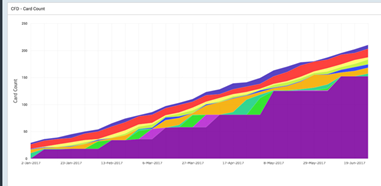
\includegraphics[width=0.5\textwidth]{flujo_acumulativo.png}
            \caption{Diagrama de flujo acumulativo.}
        \label{fig:flujo_acumulativo}
    \end{figure}
    \item \textbf{Gráfica de distribución de tiempos de ciclo:} Como se puede ver en la figura~\ref{fig:distribucion_tiempos_ciclos} es útil para ver la frecuencia con la que las tarjetas son completadas a lo largo del tiempo.
    \begin{figure}[H]
        \centering
        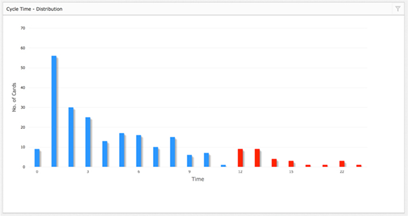
\includegraphics{distribucion_tiempos_ciclos}
        \caption{Gráfica de distribución de tiempos de ciclo.}
        \label{fig:distribucion_tiempos_ciclos}
    \end{figure}
\end{itemize}

\section{Marco tecnológico}
Para el desarrollo de este proyecto es necesario tener herramientas para las partidas con otros usuarios, así como manera de usar librerías probadas y comúnmente usadas.

\subsection{Unity3D}
Es un motor que permite diseñar videojuegos. Permite usar C\# para programar el juego, compilando, usando Mono\cite{unity2019}. Es un motor muy capaz que permite desarrollar videojuegos 2D y 3D, con una variedad de herramientas para facilitar el desarrollo (figura~\ref{fig:unity_screenshot}).

\begin{figure}[H]
    \centering
    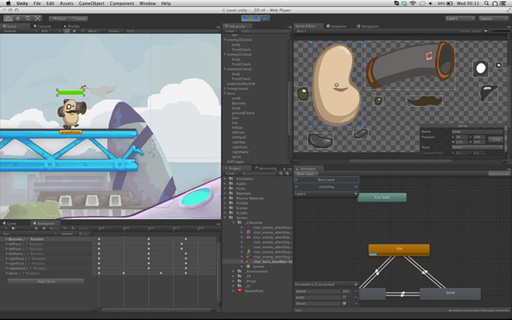
\includegraphics{unity}
        \caption{Algunas capacidades de Unity para el desarrollo de videojuegos: animaciones, máquina de estados y un editor de sprites.}
        \label{fig:unity_screenshot}
\end{figure}

Unity puede crear el juego para varios entornos, como consolas de videojuegos como la Nintento Switch, el Xbox One, PS4, Windows, MacOS, Linux, Android, iOS, o la web mediante WebGL [24].

\subsection{\textit{Mirror}}
\textit{Mirror} es una librería para crear juegos multijugador de \textit{Unity}. Es una continuación a \textit{Unet} de \textit{Unity Technologies}. Permite desarrollar el cliente y el servidor en un único proyecto.

\subsection{Git}
Git es el sistema de control de versiones más popular del mundo, fue creado en 2005 por Linus Torvalds [27]. Es un ejemplo de un \textit{DVCS}, un sistema distribuido de control de versiones. A diferencia de sistemas donde en un solo lugar esta todo el historial de versiones como \textit{CVS} o \textit{Subversion}. En \textit{Git} todas las copias funcionales de código son un repositorio que contiene todo el historial de versiones.
En comparación con otros sistemas, Git está diseñado para que la creación de \textit{ramas} y \textit{tags} sean operaciones baratas, por lo tanto, rápidas.

Github es un servicio de hospedaje de repositorios Git \cite{finley2012a}. Se uso como repositorio remoto para sincronizar cambios, además de aprovechar sus funciones para crear \textit{pipelines} para \textit{Continous Integration} permitiendo probar que el juego se pueda compilar y que ningún sistema este "roto".